%!TEX root = ../munich21.tex

\begin{frame}{Point clouds}
	A data set can often be thought of as a point cloud in $\R^n$.

	\vskip 8pt

	Underlying probability distribution concentrated in a subspace.

	\vspace*{-5pt}

	\begin{center}
		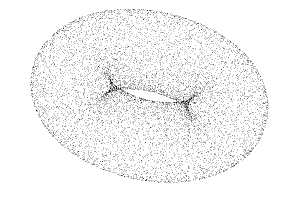
\includegraphics[scale=.3]{aux/torus}
	\end{center}

	\vspace*{-10pt} \pause

	How to approximate and study the underlying shape?

	\begin{center}
		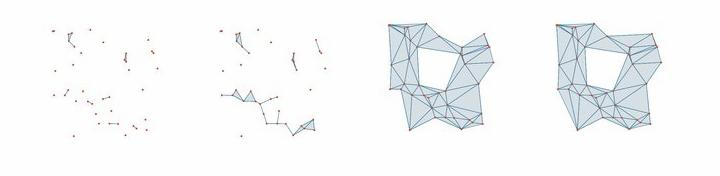
\includegraphics[scale=.4]{aux/filtration}
	\end{center}

	\vskip-15pt
	\textcolor{pblue}{Multi-scale approximation:} $X_1 \to X_2 \to \dots \to X_n$
\end{frame}

\begin{frame}{Persistence cohomology}

	\textcolor{pblue}{Barcode:}
	Quantifies ranks of all linear maps $H^n(X_j) \to H^n(X_i)$ for $i \leq j$.

	\pause
	\begin{center}
		\includegraphics[scale=.25]{aux/barcode.pdf}
	\end{center}

	\pause
	\textcolor{pblue}{Pipeline:}
	\begin{center}
		\includegraphics[scale=.8]{aux/diagram.pdf}
	\end{center}
\end{frame}

\begin{frame}[fragile]{Steenrod barcodes} \pause
	Given a filtered simplicial complex $X$
	\[
	X_0 \to X_1 \to \cdots \to X_n.
	\]
	\pause
	$Sq^k$ induces an endomorphism
	\[
	\begin{tikzcd}[column sep = small]
	H^\bullet(X_n; \Ftwo) \arrow[r] & \cdots \arrow[r] & H^\bullet(X_{n-1}; \Ftwo) \arrow[r] & H^\bullet(X_0; \Ftwo) \\
	H^\bullet(X_n; \Ftwo) \arrow[u, "Sq^k"] \arrow[r] & \cdots \arrow[r] & H^\bullet(X_{n-1}; \Ftwo) \arrow[u, "Sq^k"] \arrow[r] & H^\bullet(X_0; \Ftwo) \arrow[u, "Sq^k"].
	\end{tikzcd}
	\]
	The \textcolor{pblue}{$Sq^k$ barcode} of $X$ is the barcode of $\mathrm{img}\ Sq^k$.

	\bigskip \pause

	With \textit{Umberto Lupo} and \textit{Guillaume Tauzin} from \raisebox{-1pt}{
\includegraphics[scale=.1]{aux/giotto}}'s team

	\medskip
	develop a high-performance implementation: \textcolor{pblue}{\texttt{steenroder}}.
\end{frame}

\begin{frame}{Space of conformations of $\mathrm{C_8H_{16}}$}

	Points in $\R^{24}$ (positions of $8$ carbons in $\R^3$)

	\pause \smallskip

	Computing $Sq^1$ barcode of a ``smooth component'' of this point cloud

	\smallskip

	\includegraphics[width=\textwidth]{aux/cyclo-octane_subsampled_absolute_barcodes.pdf}

	Consistent with a \textcolor{pblue}{Klein bottle} component.
\end{frame}